
\section{Architektur}

Das MultiLayer Graph System setzt sich aus mehren Komponenten zusammen die miteinander arbeiten um die gewünschten Anforderungen zu gewährleisten.
Dabei wird GE genutzt um die Graph Daten effizent im Arbeitsspeicher der Server zu verwalten und die Kommunikation der einzelnen Komponenten zu steuern.  Das TSL-Model und eine geteilte Bibliothek bieten die Basis fur die
anderen Komponenten.

In der Architektur ist der Client für das Senden von Anfragen, wie das Ausführunen eine Algorithmus oder das Laden eines Graphen, an die Proxy zuständig.
Die Proxy verarbeitet die Anfrage und koordiniert ggf. die Berechnungen der Server. Die Server kommunizieren falls nötig für ihre Berechnungen untereinander um Daten über entfernte Knoten anzufragen oder zu senden. Sobald die Anfrage fertig bearbeitet ist schickt die Proxy eine Antwort mit den enstprechnden Ergebnissen an den Client.
Eine Darstellung dieser Arbeitsweise ist in Abbildung \ref{architektur} dargestellt.

\begin{figure}
  \centering
  \begin{subfigure}[b]{1.0\textwidth}
    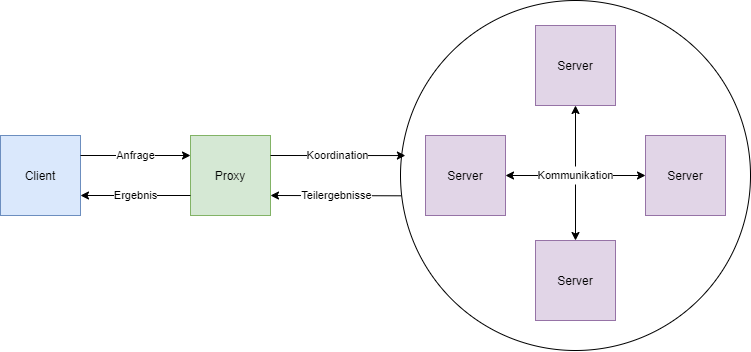
\includegraphics[width=1.0\linewidth]{img/Architektur-Cluster.png}
  \end{subfigure}
  \caption{Aufbau des Multilayer Clusters}
  \label{architektur}
\end{figure}



\subsection{Model}

Das TSL Model dient als Basis für den Rest der Anwendung. Es wird definiert wie Knoten gespeichert werden und wie Client, Server und Proxy miteinander
kommunizieren können. Die einzelnen Komponenten müssen die von GE automatisch generierten Klassen implementiernen.


Es wird die grundlegende Graphenstruktur definiert, die genutzt wird um Multilayer Graphen darzustellen. Knoten speichern hierbei jeweils ihre ID, zu welchem Layer sie gehören
und ihre Liste an ausgehenden Kanten. Dazu kommen Daten die gebraucht werden um Algorithmen auszuführen. Die können z.B. der aktuelle PageRank Wert des Knoten sein.


\subsection{Lib}

Die geteilte Bibliothek besteht aus zwei Komponenten. Sie enthält den von TSl generierten Code und macht es so dem Client/Proxy/Server möglich darauf zuzugreifen. Der generierte Code enthält auch die abstraken Klassen für Proxy und Server. Diese werden in den enstprechnden Komponenten implementiert. 

Außerdem enthält sie eine Sammlung aus Funktionen die alle Projekte nutzen können. Insbesondere eine Interface um mit dem Graphen zu interagieren und z.B. neue Knoten anzulegen oder einem Knoten neue Kanten hinzuzufügen.
Dazu kommt die Funktionalität Ergebnisse von Algorithmen ausgeben zu lassen da dies sowohl auf dem Client als auch der Proxy möglich ist.


\subsection{Client}

Der Client stellt die Schnittstelle zwischen dem Anwender und dem Multilayer System dar. Der Client kann Anweisungen des Anwenders auf zwei Arten empfangen.
Zum einem wird ein Kommandozeilen Interface bereitgestellt mit dem der Anwender interagieren kann. Zum anderen kann dem Client eine batch Datei mit Anweisungen übergeben werden
welche nacheinander ausgeführt werden.
Hierbei besteht auch die Möglichkeit zwischen dem Interaktiven und dem Batch Modus zu wechseln.

Die Anweisungen werden interpretiert und in Anfragen an die Proxy übersetzt, welche die Anfragen dann abarbeitet.

\subsection{Proxy}

Die Proxy dient als Bindeglied zwischen dem Client und den Servern. Sie nimmt Anfragen vom Client an und sorgt dafür das diese ausgeführt werden.
Dabei koordiniert sie die Ausführung der verschiedenen Algorithmen und sendet sie die nötigen Anfragen an die Server. Wenn es nötig ist, kann gewartet werden 
bis alle Server die Anfrage abgearbeitet haben. Die Server können dabei auch ein Ergebniss zurücksenden, welches die Proxy weiter verwenden kann. Ein häufiger Fall
ist hierbei das die Ergbenisse der einzelnen Server aggregiert werden.


Abhänging von der Client Anfrage ist die Proxy auch für das Messen der Laufzeit und das Bilden der Ergebnisse verantwortlich. Die Ergebnisse können im gewünschten Format entweder direkt auf der Proxy ausgegeben
oder zurück an den Client gesendet werden.

\subsection{Server}

Die Server erfüllen zwei Aufgaben. Sie verwalten sie die Graph Daten in GE und
sie warten darauf das sie Anweisungen von der Proxy bekommen und führen auf ihre Anweisung Berechnungen durch. Bei diesen Berechnungen kümmert sich jeder Server 
um die eigenen lokal gespeicherten Knoten. Die Serven können aber auch miteinander kommunizieren, wenn sie die Daten entfernter Knoten benötigen oder die Daten entfernter Knoten
aktualisieren müssen.
Ist ein Server mit einer angeforderten Aufgabe fertig kann er dies der Proxy melden. Dabei kann, falls nötig, auch ein Ergebniss mitgesendet werden.



